\chapter{Weitere Prinzipien}
\section{Analyse GRASP: Geringe Kopplung}
\textbf{Geringe Kopplung} ist ein Prinzip von GRASP, das auf die Minimierung der Abhängigkeiten zwischen Klassen oder Modulen abzielt. Es ist eine grundlegende Strategie zur Steigerung der Modulierbarkeit und Wiederverwendbarkeit von Software. Bei geringer Kopplung sind einzelne Komponenten weniger auf die internen Eigenschaften und das Verhalten anderer Komponenten angewiesen. Dies erleichtert das Verständnis des Systems, da jede Komponente einzeln verstanden werden kann. Zudem wird dadurch die Wartbarkeit verbessert, da Änderungen an einer Komponente weniger wahrscheinlich Auswirkungen auf andere haben. Geringe Kopplung erleichtert auch das Testen von Komponenten, da diese unabhängig voneinander getestet werden können.
\subsection{Positiv Beispiel}
\begin{figure}[ht]
    \centering
    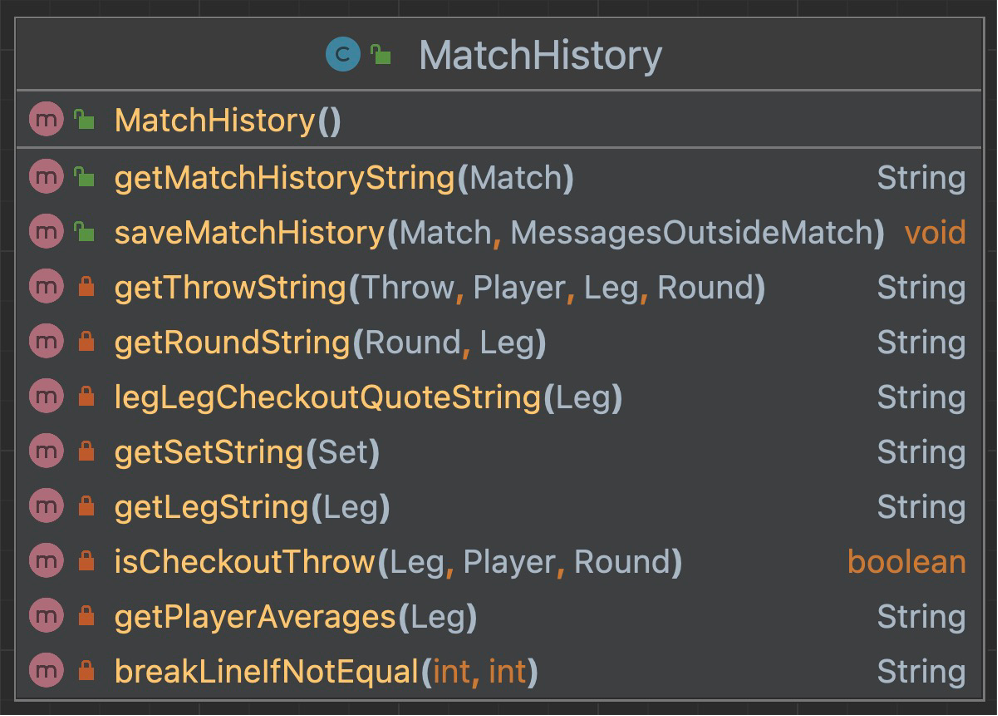
\includegraphics[width=0.7\linewidth]{Bilder/MatchHistoryUML.png}
    \caption{MatchHistory geringe Kopplung Positiv Beispiel}
    \label{fig:matchhistory-uml}
\end{figure}
Die Klasse \textit{MatchHistory} ist ein gutes Beispiel für geringe Kopplung in der Softwareentwicklung. Sie hat keine Abhängigkeiten zu anderen Klassen und kann somit unabhängig existieren und betrieben werden. Durch ihre Eigenständigkeit kann sie in jedem Moment des Programms ausgeführt oder ignoriert werden. Zum Beispiel kann der Benutzer am Ende des Programms entscheiden, ob die Match History gespeichert werden soll oder nicht. Ihre Funktionalität ist durch öffentliche Methoden wie \textit{getMatchHistoryString(Match)} und \textit{saveMatchHistory(Match, MessagesOutsideMatch)} sowie private Methoden definiert, die spezifische Aufgaben erfüllen. Alle diese Methoden sind speziell auf die Verarbeitung und Speicherung von Match-Daten zugeschnitten, und benötigen keine Kenntnisse oder Interaktionen mit anderen Teilen des Systems. Dies trägt dazu bei, die Kopplung zu minimieren und die Wartbarkeit und Erweiterbarkeit des Codes zu verbessern.

\subsection{Negativ Beispiel}
\begin{figure}[ht]
    \centering
    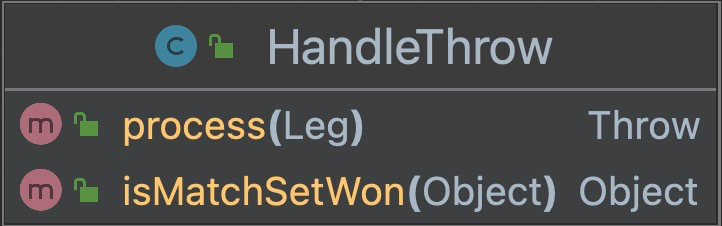
\includegraphics[width=0.7\linewidth]{Bilder/HandleThrowUML.png}
    \caption{HandleThrow geringe Kopplung Negativ Beispiel}
    \label{fig:handlethrow-uml}
\end{figure}
Die \textit{HandleThrow} Klasse zeigt einen deutlichen Mangel an geringer Kopplung. Sie ist stark an mehrere andere Klassen gebunden, einschließlich \textit{Player}, \textit{Leg}, \textit{MessagesDuringMatch}, \textit{Throw}, \textit{HandleDart}, \textit{Dart} und \textit{DartStatus}. Insbesondere führt die \textit{process()} Methode Änderungen am Zustand von \textit{Player}, \textit{Leg} und \textit{Dart}-Instanzen durch und ist somit stark an das Innenleben dieser Klassen gekoppelt. Änderungen an diesen Klassen könnten dazu führen, dass auch \textit{HandleThrow} angepasst werden muss. Außerdem verlässt sie sich auf die \textit{HandleDart} Klasse für das Verarbeiten eines Dart-Wurfs, was zusätzliche Abhängigkeiten schafft. Insgesamt fehlt dieser Klasse die Unabhängigkeit und Flexibilität, die durch geringe Kopplung erreicht werden könnte, was potenzielle Probleme bei der Wartung und Erweiterung des Codes verursachen könnte. 
Es könnte Abstraktion auf die \textit{HandleThrow}-Klasse eingesetzt werden. Dieses Prinzip bietet erhebliche Vorteile in Bezug auf Kapselung und Informationssicherheit. Anstatt direkt auf die Zustände der \textit{Player}, \textit{Leg} und \textit{Dart} Klassen zuzugreifen, könnte \textit{HandleThrow} durch Implementierung von Interfaces oder abstrakten Klassen mit diesen kommunizieren. 
\section{Analyse GRASP: Hohe Kohäsion}
\textbf{Hohe Kohäsion} bezieht sich auf das GRASP-Prinzip, das besagt, dass Klassen oder Module klar definierte, eng miteinander verbundene Verantwortlichkeiten haben sollten. Dieses Prinzip zielt darauf ab, dass die innerhalb einer Klasse oder eines Moduls gruppierten Funktionen stark miteinander verbunden sein sollten, um die Stabilität, Zuverlässigkeit und Verständlichkeit des Systems zu verbessern. Hohe Kohäsion erleichtert auch die Wartung und Erweiterung des Systems, da die Auswirkungen von Änderungen innerhalb einer Klasse auf andere Klassen minimiert werden. Sie fördert auch die Wiederverwendbarkeit von Klassen, da diese spezifische und gut definierte Aufgaben haben.\newline
\begin{figure}[ht]
    \centering
    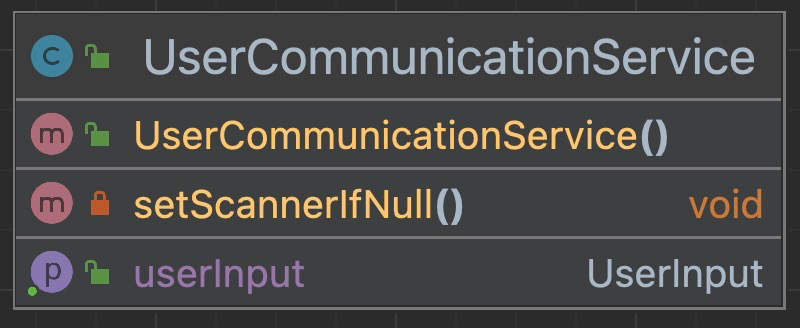
\includegraphics[width=0.7\linewidth]{Bilder/UserCommunicationServiceUML.png}
    \caption{UserCommunicationService hohe Kohäsion Positiv Beispiel}
    \label{fig:UserCommunicationService-uml}
\end{figure}\\
Die Klasse \textit{UserCommunicationService} illustriert exemplarisch das Konzept der hohen Kohäsion in der objektorientierten Softwareentwicklung. Ihr alleiniger Zweck besteht in der Verarbeitung von Benutzereingaben, welche sie in ein entsprechendes \textit{UserInput}-Objekt umwandelt und zurückgibt. Zusätzlich initialisiert diese Klasse, falls nicht bereits geschehen, einen global verfügbaren \textit{Scanner} in einer dafür bestimmten Speicherklasse. Dieses Design wurde in Anbetracht zukünftiger Erweiterungen gewählt, bei denen weitere Klassen den Scanner nutzen könnten. Zudem optimiert es die aktuelle Version im Hinblick auf Testbarkeit, indem es die Simulation von Benutzereingaben mittels Mocking erleichtert.
\section{Don't Repeat Yourself (DRY)}
\textbf{\acf{DRY}} ist ein grundlegendes Prinzip in der Softwareentwicklung, das die Eliminierung von Redundanz fördert. Das Ziel ist, dass jede Information oder jedes Verhalten im System nur an einer Stelle definiert sein sollte. Dies verringert die Fehleranfälligkeit, da bei Änderungen oder Korrekturen nur eine Stelle im Code angepasst werden muss. Es verbessert auch die Wartbarkeit, da weniger Code zu warten ist und das System einfacher zu verstehen ist. DRY fördert zudem die Konsistenz im System, da die Wahrscheinlichkeit von Inkonsistenzen durch mehrfache Definitionen reduziert wird.\\\\
Das folgende Beispiel bezieht sich auf den Commit \textbf{\href{https://github.com/P3lina/ASE-Project/commit/270423b35cf9a364a2392e71870afeed7a87e809}{270423b}}\\
\begin{figure}[ht]
    \centering
    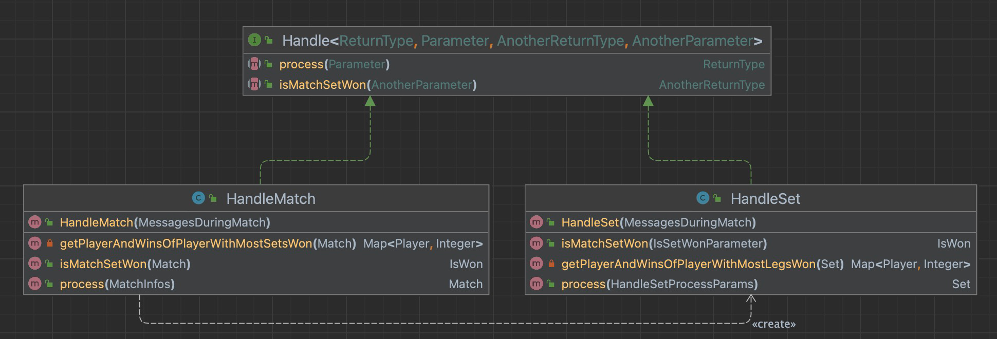
\includegraphics[width=0.85\linewidth]{Bilder/HandleDRYUML-vorher.png}
    \caption{HandleMatch und HandleSet DRY Positiv Beispiel (vorher)}
    \label{fig:handledry-vorher-uml}
\end{figure}\\
Wie in \autoref{fig:handledry-vorher-uml} zu sehen ist, enthalten die Klassen \textit{HandleMatch} und \textit{HandleSet} die nahezu gleichen Methoden \textit{isMatchSetWon} und \textit{getPlayerAndWinsOfPlayerWithMostSets}/\textit{LegsWon}. Diese beiden Methoden sind bei beiden Klassen nahezu identisch, womit knapp 50 Zeilen an Code-Duplikat existieren.\newpage
\begin{figure}[ht]
    \centering
    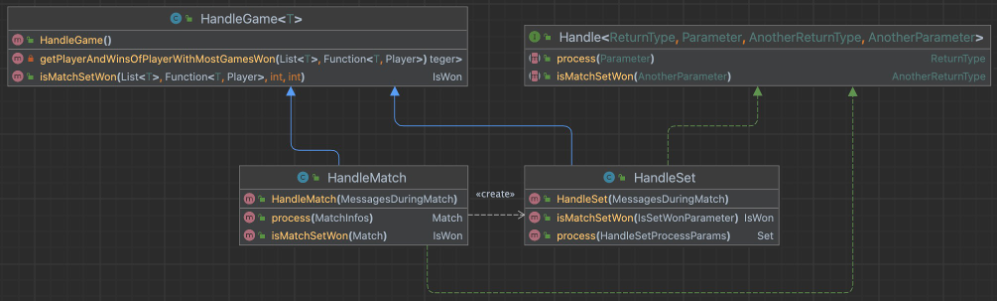
\includegraphics[width=1\linewidth]{Bilder/HandleDRYUML-nacher.png}
    \caption{HandleMatch und HandleSet DRY Positiv Beispiel (nacher)}
    \label{fig:handledry-nacher-uml}
\end{figure}
\autoref{fig:handledry-nacher-uml} zeigt, wie das Problem der doppelten Codepassagen gelöst wurde. Eine neue Klasse wurde implementiert, die als Elternklasse für die beiden vorherigen Klassen dient. Diese übergeordnete Klasse enthält die beiden Methoden, die vorher in beiden Klassen doppelt vorhanden waren.

Mit der Entfernung dieser doppelten Codepassagen lässt sich die Anzahl der Codezeilen um 50 Zeilen reduzieren. Dies trägt zur Lesbarkeit des gesamten Codes bei. Zudem zentralisiert diese Lösung die entsprechenden Methoden an einem Ort. Das erleichtert die Wartung, da bei Änderungen nur an einer Stelle Anpassungen vorgenommen werden müssen.